\documentclass[crop,tikz,10pt]{standalone}
\usepackage{tikz}
	\usetikzlibrary{shapes}
	\usetikzlibrary{automata}
	\usetikzlibrary{arrows}
	\usetikzlibrary{backgrounds}
	\usetikzlibrary{calc}
	\usetikzlibrary{positioning}
	\usetikzlibrary{patterns}
	\usetikzlibrary{shadows}
	\usetikzlibrary{decorations.pathmorphing}
	\usetikzlibrary{decorations.pathreplacing}

\usepackage[scaled]{helvet}
\renewcommand{\familydefault}{\sfdefault}

\input{../../../../../resources/latex/_symbols.qmd}

\begin{document}

\newcommand{\n}[1]{\begin{tabular}{c}#1\end{tabular}}

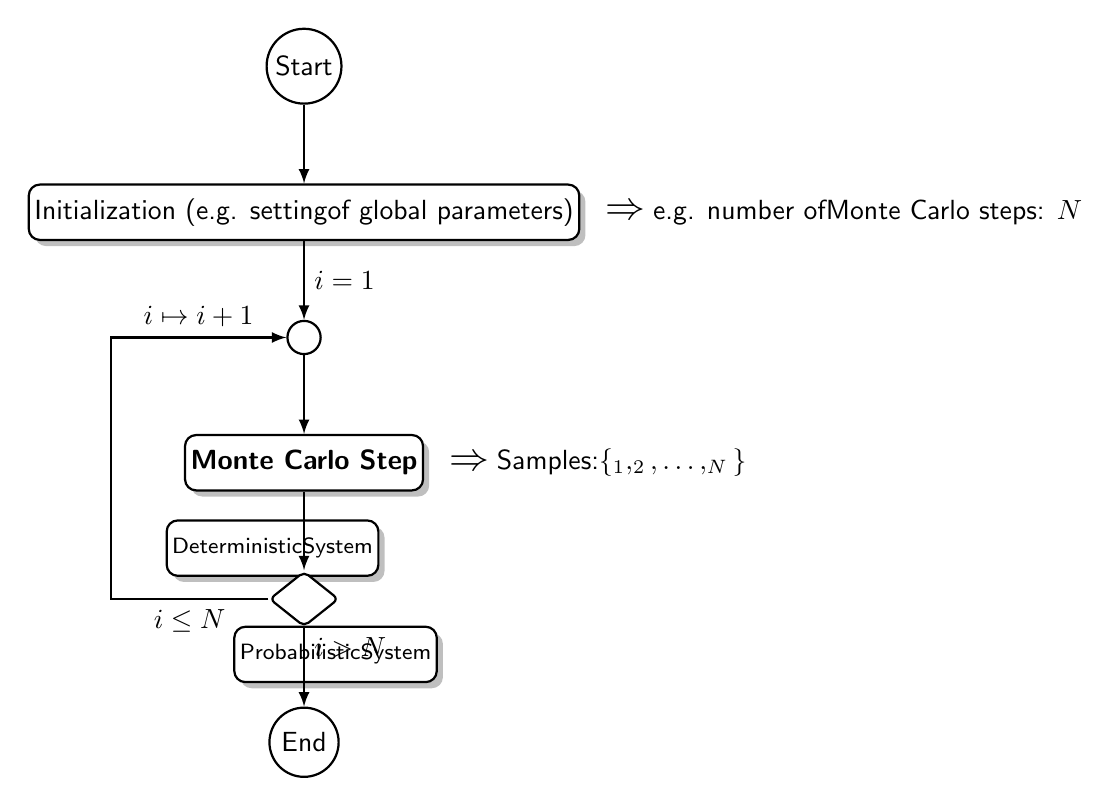
\begin{tikzpicture}[
    main/.style={draw, thick, rounded corners=4pt, inner sep=2pt, minimum size=20pt, minimum width=25pt, fill=white},
    connector/.style={draw, circle, thick, minimum size=12pt, fill=white},
    decision/.style={draw, diamond, aspect=2, thick, rounded corners=2pt, inner sep=3pt, minimum size=20pt, minimum width=25pt, fill=white},
]

    %::. main nodes
    \node[main, circle] (START) at (0,0) {\n{Start}};    
    \node[main, below = 1 of START, drop shadow] (INIT) {\n{Initialization (e.g. setting \\ of global parameters)}};
    \node[connector, below = 1 of INIT] (CON1) {};
    \node[main, below = 1 of CON1, drop shadow] (STEP) {\n{\vspace{-2mm}\\\textbf{Monte Carlo Step}\\\vspace{23mm}}};
        \node[main, drop shadow] at ($(CON1.90) - (0.4,2.9)$) {\footnotesize \n{Deterministic\\System}};
        \node[main, drop shadow] at ($(CON1.90) - (-0.4,4.25)$) {\footnotesize \n{Probabilistic\\System}};
    \node[decision, below = 1 of STEP] (DEC1) {};
    \node[main, below = 1 of DEC1, circle] (END) {\n{End}};


    \node[right = 0.2 of INIT]  {\Large$\Rightarrow$}; 
    \node[right = 0.8 of INIT]  {{\n{e.g. number of\\ Monte Carlo steps: $N$}}}; 


    \node[right = 0.2 of STEP]  {\Large$\Rightarrow$}; 
    \node[right = 0.8 of STEP] (SAMPLES) {{\n{Samples: \\ $\{\sample_1, \sample_2, \dots, \sample_N\}$ }}}; 

    
    %::. connections
    \draw[-latex, thick] (START) -- (INIT);
    \draw[-latex, thick] (INIT) -- node[midway, right] {$i=1$} (CON1);
    \draw[-latex, thick] (CON1) -- (STEP);
    \draw[-latex, thick] (STEP) --  (DEC1);
    \draw[-latex, thick] (DEC1.180) -| node [near start, below] {$i\leq N$}  ($(DEC1.180) + (-2,2)$) |- node[near end, above] {$i\mapsto i+1$} (CON1.180);
    \draw[-latex, thick] (DEC1.270) -- node[near start, right] {$i>N$} (END);
\end{tikzpicture}

\end{document}